
\begin{figure}[h]
    \caption{Markov Decision Process diagram}\label{fig:MDP}
\centering
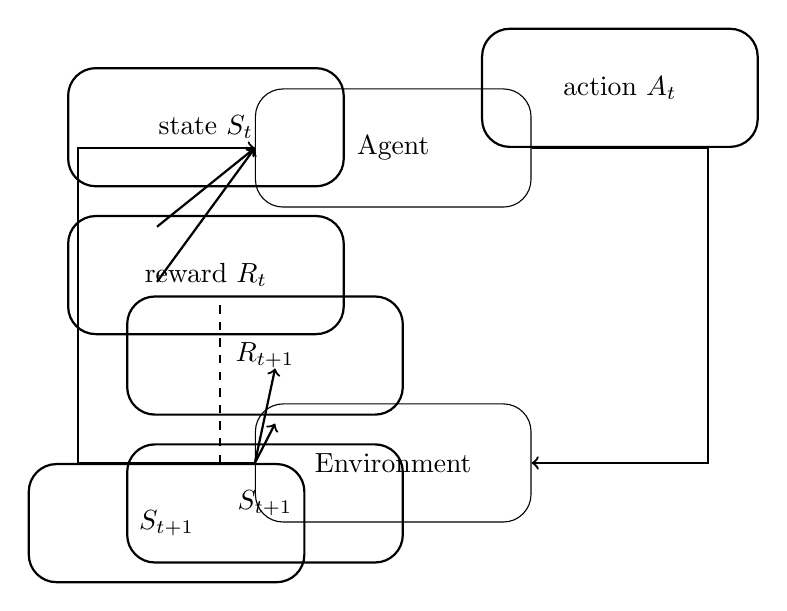
\begin{tikzpicture}[
    every node/.style={
        draw,
        rounded corners=10pt,
        minimum width=3.5cm,
        minimum height=1.5cm,
        align=center
    },
    arrow/.style={->, thick}
]

% Nodes
\node (agent) at (0,2) {Agent};
\node (env) at (0,-2) {Environment};

% Right side (action)
\draw[arrow] (agent.east) -- (4,2)
    node[midway, above] {action $A_t$}
    -- (4,-2)
    -- (env.east);

% Left outer loop (state + reward combined return)
\draw[arrow] (env.west) -- (-4,-2)
    node[midway, below] {$S_{t+1}$}
    -- (-4,2)
    -- (agent.west);

% Inner left arrows (state & reward into agent)
\draw[arrow] (-3,1) -- (agent.west)
    node[midway, above] {state $S_t$};

\draw[arrow] (-3,0.3) -- (agent.west)
    node[midway, below] {reward $R_t$};

% From environment back (split arrows)
\draw[arrow] (env.west) -- (-1.5,-1.5)
    node[midway, below] {$S_{t+1}$};

\draw[arrow] (env.west) -- (-1.5,-0.8)
    node[midway, above] {$R_{t+1}$};

% Vertical dashed line (time step separator)
\draw[dashed] (-2.2,-2) -- (-2.2,0);

\end{tikzpicture}

\caption{\textit{Markov decision process (MDP) diagram.}}
\label{fig:mdp}
\end{figure}
